% ----------------------------------------------------------
% Apêndices
% Documentos gerados pelo próprio autor
% ----------------------------------------------------------

% ---
% Inicia os apêndices
% ---
\begin{apendicesenv}

% Imprime uma página indicando o início dos apêndices
\partapendices
% ----------------------------------------------------------
\chapter{Proposta Inicial}
% ----------------------------------------------------------

\includepdf[pages=-]{EntregaFinal/PropostaInicial.pdf}

% ----------------------------------------------------------
\chapter{Sprints}
\label{sprints-atividades}
% ----------------------------------------------------------

Esta seção apresenta as atividades realizadas em cada \gls{sprint}.


\section{Sprint 1 - 10/05/2021 a 25/05/2021}

O \autoref{quadro-sprint1} mostra a divisão de tarefas da equipe durante durante o período de 10/05/2021 a 25/05/2021.

\begin{quadro}[htb]
\centering
\ABNTEXfontereduzida
\caption{Sprint 1 - 10/05/2021 a 25/05/2021}
\label{quadro-sprint1}
\begin{tabular}{|l|c|c|c|}
\hline
{\thead{Atividade}} & \thead{Responsável} & \thead{Pontuação \\ estimada} & \thead{Pontuação \\ real} \\ \hline
    Concepção do Projeto & André    &  8  &  8   \\ \hline 
    Concepção do Projeto & Bianca    &  8  &  8   \\ \hline
    Concepção do Projeto & Luiz    &  8  &  8   \\ \hline
    Concepção do Projeto & Natan    &  8  &  8   \\ \hline
    Concepção do Projeto & Patrícia    &  8  &  8   \\ \hline
    Pesquisa sobre outras aplicações  & André    & 3  & 3   \\ \hline  
    \multicolumn{4}{|c|}{Proposta Inicial} \\ \hline
    Justificativa                     & Natan    &  1  &  5   \\ \hline
    Objetivo                          & Luiz     &  1  &  5   \\ \hline
    Escopo                            & Patrícia &  2  &  3   \\ \hline
    Integrações                       & André    &  1  &  1    \\ \hline   
    Tecnologia e Infraestrutura       & André    &  1  &  2    \\   \hline
    Tecnologia e Infraestrutura       & Patrícia &  1  &  2  \\ \hline
    Parcerias e Viabilidade Comercial & Patrícia &  1  &  1  \\ \hline 
    Revisão da Documentação           & Bianca   &  1  &  2  \\ \hline  
    Apresentação                      & Bianca   &  5  &  5  \\ \hline 
    \multicolumn{4}{|c|}{Blog} \\ \hline
    Postagem - Semana 01      & Bianca    & 1 &  1  \\ \hline
    Postagem - Semana 02      & Bianca     & 1 &  1 \\ \hline
\end{tabular}
\fonte{Os autores}
\end{quadro}
\FloatBarrier

\section{Sprint 2 - 25/05/2021 a 08/06/2021}
\begin{quadro}[htb]
\centering
\ABNTEXfontereduzida
\caption{Sprint 2 - 25/05/2021 a 08/06/2021}
\label{quadro-sprint2}
\begin{tabular}{|l|c|c|c|}
\hline
{\thead{Atividade}} & \thead{Responsável} & \thead{Pontuação \\ estimada} & \thead{Pontuação \\ real} \\ \hline  
    \multicolumn{4}{|c|}{Proposta Inicial} \\ \hline
    Ajustes - Justificativa           & Patrícia    & 2  & 3 \\ \hline
    Ajustes - Objetivo                & Patrícia     & 2  & 2  \\ \hline
    Detalhamento do Escopo            & Patrícia & 3 &  5 \\ \hline
    Ajustes - Escopo                  & Patrícia    & 2  & 3   \\ \hline   
    Ajustes - Análise Comparativa       & Natan    & 1  & 2   \\   \hline
    Ajustes - Análise Comparativa       & Bianca & 1 & 2 \\ \hline
    Evoluções Previstas  & Patrícia & 2  & 2   \\ \hline 
    Ajustes - Integrações          & Natan & 1 & 1   \\ \hline  
    Ajustes - Tecnologias                   & Natan & 2  & 3    \\ \hline 
    Ajustes - Tecnologias                   & Luiz & 2  & 3   \\ \hline 
    Monetização    & Bianca & 2  & 3   \\ \hline 
    Monetização    & Natan & 2  & 3   \\ \hline 
    Suporte nos Ajustes  & André & 3 & 5   \\ \hline 
    Formatação da Documentação & Patrícia & 2  & 3  \\ \hline 
    Formatação da Documentação & Luiz & 2  & 3   \\ \hline 
    Revisão da Documentação & Bianca & 1  & 2   \\ \hline 
    Ajustes - Apresentação & Bianca & 3 & 3   \\ \hline 
    
    \multicolumn{4}{|c|}{Desenho da Aplicação} \\ \hline
    Introdução  & Natan & 2 & 2   \\ \hline 
    Revisão Bibliográfica  & Natan & 5 & 5   \\ \hline 
    Arquitetura da Solução  & Patrícia & 8  & 8   \\ \hline 
    Escopo  & Patrícia & 8 & 8   \\ \hline 
    Escopo  & Bianca & 8  & 8   \\ \hline 
    Viabilidade Financeira  & Natan & 2  & 5   \\ \hline 
    Escalabilidade  & Patrícia & 3  & 2  \\ \hline 
    Segurança  & Luiz & 3 &  2  \\ \hline 
    Tecnologias  & Luiz & 3 & 3   \\ \hline 
    Manutenibilidade da aplicação  & Patrícia & 2  & 2   \\ \hline 
    Metodologias  & Bianca & 3  & 3   \\ \hline 
    Revisão da Documentação  & Luiz & 1  & 2\\ \hline 
    
    \multicolumn{4}{|c|}{Desenvolvimento do Back-End} \\ \hline
    Criar repositório no github & André & 1  &  1  \\ \hline 
    Preparação do ambiente & André & 1  &  1  \\ \hline 
    Configuração do banco de dados em produção & André & 2  & 2   \\ \hline 
    Autenticação pelo firebase & André & 2  & 2   \\ \hline 
    Fluxo de primeiro acesso & André & 3  & 3   \\ \hline 
    Teste de primeiro acesso (integração) & André & 3  & 3  \\ \hline 
    
    \multicolumn{4}{|c|}{Desenvolvimento do Front-End} \\ \hline
    Criar repositório no github & André & 1  & 1  \\ \hline 
    Criar tela de login & André & 3  & 3   \\ \hline 
    Criar tela de novo acesso & André & 3  & 3 \\ \hline 
    
    \multicolumn{4}{|c|}{Blog} \\ \hline
    Postagem - Semana 03      & Bianca    & 1  & 1    \\ \hline
    Postagem - Semana 04      & Bianca     & 1  & 1  \\ \hline
    
    \multicolumn{4}{|c|}{Vídeo} \\ \hline
    Gravar o vídeo da proposta inicial & Natan & 1  & 3   \\ \hline 
\end{tabular}
\fonte{Os autores}
\end{quadro}
\FloatBarrier

\section{Sprint 3 - 08/06/2021 a 22/06/2021}
\begin{quadro}[htb]
\centering
\ABNTEXfontereduzida
\caption{Sprint 3 - 08/06/2021 a 22/06/2021}
\label{quadro-sprint3}
\begin{tabular}{|l|c|c|c|}
\hline
{\thead{Atividade}} & \thead{Responsável} & \thead{Pontuação \\ estimada} & \thead{Pontuação \\ real} \\ \hline
    \multicolumn{4}{|c|}{Desenho da Aplicação} \\ \hline
    Ajustes - Lista de Siglas           & Natan    & 2  & 3   \\ \hline
    Ajustes - Introdução                          & Natan & 2 & 2  \\ \hline
    Ajustes - Arquitetura de Solução              & Patrícia & 2 & 2  \\ \hline
    Ajustes - Escopo                       & Bianca    & 3  & 3    \\ \hline   
    Ajustes - Viabilidade Financeira       & Natan    & 2  &    3\\   \hline
    Ajustes - Metodologias       & Bianca & 2 & 2 \\ \hline
    Ajustes - Product Backlog & Patrícia & 2  & 2   \\ \hline 
    Revisão da Documentação           & Natan & 1  & 2   \\ \hline  
    Configuração do LaTeX diff           & Natan & 1  & 3   \\ \hline 
    Apresentação 		 & Bianca & 5  & 5    \\ \hline
    
     \multicolumn{4}{|c|}{Histórias de Usuário} \\ \hline
     Administrador & André & 5  & 8   \\ \hline
     Gestor & Luiz & 5  & 8   \\ \hline
     Professor & Bianca & 8  & 8   \\ \hline
     Aluno & Patrícia & 8  & 8    \\ \hline
     Criar mais histórias de usuário & Patrícia & 8  & 8   \\ \hline
    
    \multicolumn{4}{|c|}{Desenvolvimento do Back-End} \\ \hline
    Autenticação e Autorização & André & 1  &  2  \\ \hline 
    Cadastro e Visualização do Administrador & André & 2  &  2  \\ \hline 
    Envio de e-mail do primeiro acesso & André & 1  & 2   \\ \hline 
    
    \multicolumn{4}{|c|}{Desenvolvimento do Front-End} \\ \hline
    Elaboração de Protótipos de baixa fidelidade & André & 3  & 5  \\ \hline 
    Elaboração de Protótipos de baixa fidelidade & Luiz & 3  & 5   \\ \hline 
    
    \multicolumn{4}{|c|}{Blog} \\ \hline
    Postagem - Semana 05      & Bianca    & 1  & 1    \\ \hline
    Postagem - Semana 06      & Bianca     & 1 & 1  \\ \hline
    
    \multicolumn{4}{|c|}{Vídeo} \\ \hline
    Gource & Natan & 1  &  2  \\ \hline
    
\end{tabular}
\fonte{Os autores}
\end{quadro}
\FloatBarrier

\section{Sprint 4 - 22/06/2021 a 06/07/2021}
\begin{quadro}[htb]
\centering
\ABNTEXfontereduzida
\caption{Sprint 4 - 22/06/2021 a 06/07/2021}
\label{quadro-sprint4}
\begin{tabular}{|l|c|c|c|}
\hline
{\thead{Atividade}} & \thead{Responsável} & \thead{Pontuação \\ estimada} & \thead{Pontuação \\ real} \\ \hline
    \multicolumn{4}{|c|}{Desenho da Aplicação} \\ \hline
    Tag SVN           & Natan    & 2  & 3   \\ \hline
    \multicolumn{4}{|c|}{Prova de Conceito} \\ \hline
    Ajustes no código                     & André    & 5  & 5   \\ \hline
    Subir no SVN                          & Bianca & 1 & 1  \\ \hline
    Apresentação                            & André & 5 & 5  \\ \hline
    Relatório                       & André    & 5  & 8   \\ \hline   
    Formatação LaTeX       & Natan    & 2  & 3     \\   \hline
    Vídeo       & Natan & 2 & 3  \\ \hline
    Desenhar arquitetura & Patrícia & 8  & 8   \\ \hline 
    Tags SVN           & Natan & 1  & 3    \\ \hline  
    
    \multicolumn{4}{|c|}{Desenvolvimento do Back-End} \\ \hline
    Criar listagem e paginação de administradores cadastrados & André    & 5  & 8   \\ \hline   
    Arrumar fluxo de login e primeiro acesso & André    & 5  & 8   \\ \hline 
    Criar cadastro de escolas & André    & 5  & 8   \\ \hline   
    Aumentar cobertura de testes & André    & 5  & 8   \\ \hline  
    Exclusão de administradores & Patrícia & 3  & 5   \\ \hline 
    
    \multicolumn{4}{|c|}{Desenvolvimento do Front-End} \\ \hline
    Criar tela de cadastro de escolas & André    & 5  & 8   \\ \hline 
    Elaboração de Protótipos de alta fidelidade & Patrícia & 3  & 5   \\ \hline 
    Elaboração de Protótipos de alta fidelidade & Luiz & 3  & 5   \\ \hline 
    
    \multicolumn{4}{|c|}{Blog} \\ \hline
    Ajustes no conteúdo  & Bianca    & 1  & 1    \\ \hline
    Postagem - Semana 07      & Bianca    & 1  & 1    \\ \hline
    Postagem - Semana 08      & Bianca     & 1 & 1   \\ \hline
    
    \multicolumn{4}{|c|}{Vídeo} \\ \hline
    Gource (POC) & Natan &  1 &  1  \\ \hline 
    Gravação do vídeo (Desenho da Aplicação) & Bianca & 1 & 1    \\ \hline
    Gravação do vídeo (Desenho da Aplicação) & Luiz & 1  & 1    \\ \hline
    Gravação do vídeo (Desenho da Aplicação) & Natan & 1  & 1    \\ \hline
    Gravação do vídeo (Desenho da Aplicação) & Patrícia & 1  & 1    \\ \hline
    
    \multicolumn{4}{|c|}{LaTeX} \\ \hline
    Adequação dos arquivos em LaTeX & Natan & 3 & 5   \\ \hline 
    Subir no SVN & Natan & 1 & 1   \\ \hline
    
\end{tabular}
\fonte{Os autores}
\end{quadro}
\FloatBarrier

\section{Sprint 5 - 06/07/2021 a 20/07/2021}
\begin{quadro}[htb]
\centering
\ABNTEXfontereduzida
\caption{Sprint 5 - 06/07/2021 a 20/07/2021}
\label{quadro-sprint5}
\begin{tabular}{|l|c|c|c|}
\hline
{\thead{Atividade}} & \thead{Responsável} & \thead{Pontuação \\ estimada} & \thead{Pontuação \\ real} \\ \hline
    \multicolumn{4}{|c|}{Documentação Final} \\ \hline
    Ajustes na estrutura do documento & Bianca & 5  & 8  \\ \hline
    Ajustes - Revisão de Literatura & Bianca & 1  & 2   \\ \hline 
    Atividades das sprints       & Bianca & 1 & 5  \\ \hline
    Postagens do blog  & Bianca & 1 & 2  \\ \hline
    Métricas do projeto  & Bianca    & 1  & 5   \\ \hline   
    Proposta Inicial  & Bianca    & 1  & 1   \\ \hline  
    QR Codes       & Luiz    & 1  & 1     \\   \hline
    QR Codes       & Natan    & 1  & 1     \\   \hline
    Escolhas e Descartes       & Luiz & 1 & 2  \\ \hline
    Escolhas e Descartes & Bianca & 1  & 1   \\ \hline 
    Ajustes - Escopo & Bianca & 1  & 3   \\ \hline 
    Modelagem de Dados & Natan & 1  & 3   \\ \hline 
    Testes Front-end & Patricia & 1  & 1   \\ \hline 
    Testes Back-end & Bianca & 1  & 1   \\ \hline 
    Entregáveis & Bianca & 1  & 1   \\ \hline 
    Ajustes - Segurança & Bianca & 1  & 1   \\ \hline 
    Considerações Finais   & Bianca & 2  & 5    \\ \hline  
    
    \multicolumn{4}{|c|}{Desenvolvimento do Back-End} \\ \hline
    Cadastro de conquista & André    & 5  & 5   \\ \hline  
    Entrega de conquista & André    & 5  & 8   \\ \hline 
    CRUD de gestores & André & 3  & 5    \\ \hline  
    CRUD de alunos & André & 3  & 5    \\ \hline  
    CRUD de professores & André & 3  & 8    \\ \hline 
    Endpoint cadastro de turma & André    & 3  & 3   \\ \hline
    Endpoint cadastro de atividades & André    & 3  & 3   \\ \hline  
    Busca dinâmica de escolas & Natan & 3  & 3   \\ \hline 
    Busca dinâmica de administradores & Natan & 3  & 3   \\ \hline 
    Busca dinâmica de gestores & Natan & 3  & 3   \\ \hline 
    Busca dinâmica de professores & Natan & 3  & 3   \\ \hline
    Criação dos loaders & Gustavo & 3  & 5   \\ \hline 
    Traduções dos placeholders & Gustavo & 2  & 5   \\ \hline 
    Tratamento de erros nos formulários & Gustavo & 3  & 5   \\ \hline 
    Aumentar cobertura de testes & André    & 3  & 5   \\ \hline 
    
    \multicolumn{4}{|c|}{Desenvolvimento do Front-End} \\ \hline
    Configuração do Cypress & André    & 1  & 3   \\ \hline 
    Tela do cadastro de turmas & André & 3  & 3   \\ \hline 
    Tela do cadastro de atividades & André & 3  & 3   \\ \hline
    Listagem de turmas & André & 2  & 2   \\ \hline 
    Visão do professor & André & 5  & 8   \\ \hline 
    Tela de criação de professor & Gustavo & 3  & 5   \\ \hline 
    Testes de Escolas & Patricia & 2  & 5   \\ \hline 
    Testes de Administradores & Patricia & 2  & 5   \\ \hline 
    Testes de Gestores & Patricia & 2  & 5   \\ \hline 
    Testes de Professores & Patricia & 2  & 5   \\ \hline 
    Configurar relatórios de testes & Patricia & 2  & 3   \\ \hline 
    Estilização de telas & Patricia & 3  & 5   \\ \hline 
    
    \multicolumn{4}{|c|}{Blog} \\ \hline
    Postagem - Semana 09      & Bianca    & 1  & 1    \\ \hline
    Postagem - Semana 10      & Bianca     & 1 & 1   \\ \hline
    
    \multicolumn{4}{|c|}{Vídeo} \\ \hline
    Gource (POC) & Natan & 1  &  1  \\ \hline 
    
    
\end{tabular}
\fonte{Os autores}
\end{quadro}
\FloatBarrier

% ----------------------------------------------------------
\chapter{Publicações do Blog}
% ----------------------------------------------------------

Ao longo do desenvolvimento do projeto, foram feitas postagens semanais no blog a respeito das atividades exercidas por cada integrante, sobre as reuniões realizadas e decisões tomadas pela equipe.

\section{Resumo de Atividades - Semana 1}

Esse blog tem como objetivo mostrar um acompanhamento semanal do projeto que estamos desenvolvendo para a disciplina de Projeto Integrado I (PI1A5).

Na primeira semana, definimos os integrantes da equipe:

\begin{itemize}
\item André Monteiro Gomes;
\item Bianca Kaori Hng;
\item Luiz Henrique de Almeida e Albuquerque;
\item Natan da Fonseca Lisboa;
\item Patricia Santos Paschoal.
\end{itemize}

E como ideia principal foi decidido que seria algo voltado para a educação, devido à proximidade de alguns dos integrantes com a área e também devido ao fato de já houver alguns esboços de ideias relacionados a isso pelos próprios integrantes. 

A metodologia de gestão adotada foi o Scrum e a gerente do projeto escolhida fui eu, Bianca.

Então, a Patrícia começou a elicitar possíveis requisitos para a aplicação e o André, possíveis tecnologias a serem usadas.

O nome escolhido para a equipe foi "DevAneios", sugerido pelo Natan e, para o nome do projeto, foi escolhido "Turma de Elite", sugerido pelo Luiz. E eu, Bianca, criei o canal do YouTube e o Blog para o projeto.

Fizemos uma reunião com todos os integrantes e, assim, ficou decidido que o projeto aplicaria conceitos de gamificação para a execução de atividades, com o objetivo de incentivar os alunos a desenvolverem as tarefas.


\section{Resumo de Atividades - Semana 2}
Apresentamos a ideia do projeto para o professor e esta foi aceita por ele com a orientação de aprofundá-la para a apresentação da próxima semana. 

Então, a segunda semana foi dedicada ao amadurecimento da ideia e a elaboração do documento e a apresentação da proposta inicial para a turma. 

Nos reunimos duas vezes ao longo da semana: a primeira para amadurecer a ideia do projeto, tanto as funcionalidades que o sistema terá, quanto as tecnologias que serão utilizadas, e também para definir os próximos passos de cada um; e a segunda reunião foi para o alinhamento da equipe para a apresentação da proposta inicial.

Assim, ficou decidido que a aplicação teria um módulo para as atividades, painel de conquistas, ranking dos alunos por liga e \glspl{dashboard} para acompanhamento.
Segue abaixo as atividades de cada integrante:

\begin{itemize}
\item André: trouxe as ideias para o aperfeiçoamento do projeto, pesquisa sobre outras aplicações e fez a elaboração da documentação (integração e tecnologias utilizadas);
\item Bianca: fez a elaboração da apresentação, revisão da documentação e ficou responsável pelas postagens semanais no blog;
\item Luiz: fez a elaboração da documentação (objetivo);
\item Natan: fez a elaboração (justificativa) e revisão da documentação, e a sua conversão para LaTeX;
\item Patricia: fez a elaboração da documentação (escopo, parcerias e tecnologias utilizadas) e mapeamento das funcionalidades da aplicação.
\end{itemize}

\section{Resumo de Atividades - Semana 3}
Apresentamos a proposta inicial para o professor e aos demais alunos da turma. E com o \gls{feedback} do professor, nos reunimos para estabelecer os principais pontos apontados por ele e dividimos as tarefas para cada um.

Para facilitar a comunicação entre os integrantes da equipe e ver o andamento do projeto, foi decidido que uma vez por semana a equipe se reuniria para os \glspl{checkpoint} semanais. O dia escolhido foi terça-feira às 19h30 pois era o melhor dia e horário para todos os integrantes. 

Então, a terceira semana foi dedicada aos ajustes da apresentação e da documentação da proposta inicial e também ao início do desenvolvimento da aplicação.

Segue abaixo as atividades de cada integrante:

\begin{itemize}
\item André: focou na parte de desenvolvimento da aplicação, então criou uma organização no \gls{github}, fez a implementação da autenticação, preparação do \ac{ci} e preparação dos ambientes para receber a aplicação, e também prestou suporte para a documentação;
\item Bianca: fez os ajustes da documentação (análise comparativa e monetização) e da apresentação, bem como a revisão da documentação da proposta inicial, além da preparação de arquivos para a gestão do projeto e criação do equipe.yaml;
\item Luiz: fez os ajustes da documentação (tecnologias) e auxiliou na formatação da documentação da proposta inicial;
\item Natan: fez os ajustes da documentação (análise comparativa, integrações, tecnologias e monetização), auxiliou na sua formatação e fez a gravação e postagem do vídeo de apresentação da proposta inicial;
\item Patrícia: fez os ajustes (evoluções previstas), o melhoramento (justificativa e objetivo) e a formatação da documentação da proposta inicial, bem como o detalhamento do escopo.
\end{itemize}

\section{Resumo de Atividades - Semana 4}
Tivemos uma reunião para acompanhamento do projeto e eventuais dúvidas com o professor e também tivemos uma reunião de \gls{checkpoint} e definição de próximos passos para o projeto, no qual foi definido que focaríamos no desenho da aplicação e no desenvolvimento inicial dos testes.

Então, a quarta semana foi dedicada à elaboração do desenho e início da implementação dos testes. 

Segue abaixo as atividades de cada integrante:

\begin{itemize}
\item André: fez a implementação de autenticação/autorização com Firebase Authentication, criação de \gls{setup} para teste de integração e a integração com ferramentas de análise estática (Deepsource e Eslint);
\item Bianca: fez a elaboração do desenho da aplicação, fazendo a parte de metodologias e escopo, além da revisão do desenho;
\item Luiz: fez a elaboração do desenho da aplicação, fazendo a parte de segurança e tecnologias, e revisão da documentação ;
\item Natan: fez a elaboração do desenho da aplicação, fazendo a parte da introdução, revisão bibliográfica e viabilidade financeira;
\item Patricia: fez a elaboração do desenho da aplicação, fazendo a parte da arquitetura de solução, escopo, escalabilidade e manutenibilidade da aplicação.
\end{itemize}

\section{Resumo de Atividades - Semana 5}
Na quinta semana, tivemos uma reunião de acompanhamento com o professor e mostramos o desenho de aplicação a ele. E, ao longo dessa reunião, ele apontou alguns pontos de melhoria.

Decidimos levar mais a sério a metodologia adotada, então na reunião semanal da equipe, tratamos de marcar todas as entregas que tivemos na \gls{sprint} (Sprint Review) e o que podia ser melhorado (Sprint Retrospective). Um dos pontos levantados para melhoria foi a falta de uma definição clara do projeto. Então, como plano de ação, decidimos levantar as histórias de usuário, para a partir disso sabermos se todos estavam alinhados com as funcionalidades do projeto. 

Dividimos as histórias por tipos de usuários para cada um e, depois de escritas, nos reunimos mais uma vez para discutirmos o que fazia parte do escopo e o que não.

Em paralelo, foram configurados os vídeos do Gource e com isso mostrou-se necessário uma logo para o projeto.

Além disso, foram feitos os ajustes no desenho do projeto, a preparação da apresentação dele e a preparação para a \ac{poc}.

Segue abaixo as atividades de cada integrante:

\begin{itemize}
\item André: configurou o Firebase em produção, implementou testes integrados com Firebase Emulator e escreveu as histórias de usuário do administrador;
\item Bianca: escreveu as histórias de usuário do professor, fez os ajustes no desenho da aplicação (metodologia e modelagem da aplicação) e fez a elaboração da apresentação do desenho;
\item Luiz: fez a elaboração de vários logos para ser escolhida pela equipe, melhorou aquela que foi mais votada e escreveu as histórias de usuário do gestor;
\item Natan: colocou a lista de siglas e o glossário no desenho da aplicação, revisou e criou o latexdiff nele, alterou a parte da introdução e da viabilidade financeira e configurou os vídeos do Gource;
\item Patricia: escreveu as histórias de usuário do aluno e reescreveu a escalabilidade, arquitetura da solução, padrão do projeto e \gls{coding-convention} do desenho da aplicação.
\end{itemize}

\section{Resumo de Atividades - Semana 6}
Assistimos as apresentações do desenho do projeto das outras equipes e, com os \glspl{feedback} do professor para eles, anotamos o que precisaria alterar no nosso desenho. Então, a sexta semana teve como principal foco as mudanças no desenho da aplicação, principalmente na modelagem do projeto. E também tratamos do relatório de avaliação das outras equipes.

Além disso, nos reunimos para o \gls{checkpoint} semanal e nele decidimos fazer um acompanhamento diário das atividades, visto que, desse modo, conseguiríamos ter uma melhor visualização das atividades ao longo da semana. Por isso, criamos uma página no Notion para fazermos a nossa \textit{Daily}.

E, na parte de códigos, focamos no desenvolvimento da \ac{poc}, corremos atrás para validar se todos os pontos dela foram cumpridos e também lidamos com o desenvolvimento dos testes e questões de segurança.

Segue abaixo as atividades de cada integrante:

\begin{itemize}
\item André: desenvolveu a \ac{poc}, iniciou os protótipos de baixa fidelidade, fez os testes de integração para autenticação e melhorou a nota no securityheaders.com;
\item Bianca: criou a página no Notion, fez o relatório da avaliação das outras equipes (ConsacreTADS) e alterou o desenho do projeto (metodologia e escopo) e a apresentação;
\item Luiz: iniciou os protótipos de alta fidelidade
Natan: fez a \gls{checklist} das tarefas da \ac{poc} e da aplicação, fez o relatório de avaliação das outras equipes (AcadTech) e ajustou a formatação do desenho da aplicação;
\item Patricia: criou mais histórias de usuários, fez o mapeamento delas por funcionalidade e ordem de importância, gerando assim o \gls{product-backlog} mais atualizado.
\end{itemize}

\section{Resumo de Atividades - Semana 7}
Na sétima semana, apresentamos o desenho da aplicação para o professor e para os demais alunos da turma. E anotamos o feedback do professor, sob a orientação dele de manter o desenho da aplicação como estava no \ac{svn} e melhorá-lo para a documentação final.

Então, no nosso checkpoint semanal, decidimos focar na \ac{poc}, nos protótipos da aplicação e nas entregas gerais do projeto para a disciplina. E também gravamos vídeos para postar no YouTube.

Segue abaixo as atividades de cada integrante:

\begin{itemize}
\item André: criou a listagem e a paginação de administradores cadastrados, consertou o fluxo de login e primeiro acesso, subiu a versão de \gls{release} para a apresentação da \ac{poc} e fez o relatório e apresentação dela;
\item Bianca: gravou o vídeo da apresentação do desenho do projeto, começou a alterar o modelo lógico da aplicação, alterou o equipe.yaml para colocar as \ac{url}s que faltavam e fez a revisão do relatório da \ac{poc};
\item Luiz: gravou o vídeo da apresentação do desenho do projeto e começou a elaboração dos protótipos de alta fidelidade;
\item Natan: gravou o vídeo da apresentação do desenho do projeto e da prova de conceito, fez sua edição e postagem no YouTube, gerou o vídeo do Gource e adicionou as tags no \ac{svn} até o desenho do projeto ;
\item Patricia: fez os protótipos a nível \gls{wireframe} da visão do aluno, gravou o vídeo da apresentação do desenho do projeto, fez a prototipação de alta fidelidade das telas de login e visão do aluno e fez a modelagem de diagramas para a \ac{poc}.
\end{itemize}

\section{Resumo de Atividades - Semana 8}
Na oitava semana apresentamos a prova de conceito para o professor e para os demais alunos da turma.

Ao longo da semana, nos reunimos para o \gls{checkpoint} semanal e nele foi decidido que toda a equipe direcionaria seus esforços para o desenvolvimento da aplicação.

Então, tivemos uma reunião de alinhamento de código, na qual foi explicado sua estrutura e como configurar na máquina local, bem como a definição dos próximos passos.

Além disso, foram feitos ajustes gerais na documentação e no \ac{svn}.

Segue abaixo as atividades de cada integrante:

\begin{itemize}
\item André: aumentou a cobertura de testes do sistema, conduziu a reunião de alinhamento do código e criou cadastro de escolas no \glspl{back-end};
\item Bianca: iniciou a escrita da documentação final, configurou o projeto para rodar em máquina local e fez edição de escolas;
\item Luiz: fez a prototipação de alta fidelidade da visão do professor;
\item Natan: fez os ajustes da estrutura de arquivos da documentação LaTeX no Overleaf, atualizou as \textit{tags} no repositório e fez o relatório de avaliação da apresentação da prova de conceito das outras equipes; 
\item Patricia: fez a prototipação de alta fidelidade da visão do gestor, configurou o projeto para rodar em máquina local e criou a exclusão de administradores no \glspl{back-end}.
\end{itemize}

\section{Resumo de Atividades - Semana 9}
Na nona semana ficamos sabendo que um dos grupos da sala seria desfeito devido ao fato de que duas integrantes trancariam a disciplina. Então, os outros três integrantes foram alocados nas outras equipes e assim o Gustavo entrou para a nossa equipe :)

Desse modo, a semana foi dedicada em passar as principais informações a respeito do projeto ao novo integrante, além do desenvolvimento da aplicação e da documentação final.

A nossa reunião semanal foi voltada a uma retrospectiva do projeto, na qual todos os integrantes falaram o que estavam achando em relação ao projeto, o que estavam gostando e o que não estavam gostando, de modo a saber se todos os integrantes estavam alinhados e satisfeitos com o desenvolvimento do mesmo. Foi uma reunião leve e como principal ponto de insatisfação levantado foi o grande escopo. Por isso, como plano de ação, foi decidido que a visão do \gls{ranking} será menos detalhada, as conquistas serão travadas, e turma e disciplina serão a mesma coisa.

Segue abaixo as atividades de cada integrante:

\begin{itemize}
\item André: adicionou a edição dos usuários, criou operações \ac{crud} para o gestor e para o professor, criou o esboço para o cadastro e entrega de conquistas e aumentou a cobertura de testes;
\item Bianca: focou na documentação final, ajustando a estrutura do documento, colocou as postagens do blog, as atividades das \glspl{sprint} e os protótipos da tela e iniciou as métricas do projeto;
\item Gustavo: criou a página de criação do professor pela visão do gestor e fez correções dos textos exibidos nessa página;
\item Luiz: focou na documentação final, criando os \glspl{qr-code} para os links da aplicação e escrevendo as escolhas e os descartes;
\item Natan: gerou o vídeo do Gource até a prova de conceito e postou no YouTube, adicionou os custos do banco de dados e escreveu \glspl{link} de acesso no documento final;
\item Patricia: fez a estilização da tela de envio de \gls{link} de \gls{reset} de senha, tentou desenvolver testes unitários no front-end e configurou o protractor para testes e2e.
\end{itemize}

\section{Resumo de Atividades - Semana 10}
Na décima semana, apresentamos ao professor o andamento da documentação final e do desenvolvimento da aplicação. Tiramos algumas de nossas dúvidas e ele fez algumas sugestões de melhoria e alguns pontos de atenção.

No nosso checkpoint semanal, foi decidido que a maioria da equipe focaria no desenvolvimento da aplicação, enquanto apenas dois integrantes cuidariam da documentação final. Entretanto, devido a contratempos que surgiram ao longo da semana, foi necessária a ajuda de quase toda a equipe na elaboração do documento final no final da semana.

Segue abaixo as atividades de cada integrante:
\begin{itemize}
\item André: configurou o Cypress, fez o CRUD de alunos, criou a tela e o endpoint para cadastro de turmas, criou a listagem de turmas e a visão do professor, além de criar a tela e o endpoint para cadastro de atividades
\item Bianca: focou na documentação final (análise de requisitos, considerações finais e métricas), além de ajustar a estrutura e revisar o documento 
\item Gustavo: fez a criação dos loaders, iniciou as traduções dos placeholders e o tratamento de erros no formulário, além de auxiliar na documentação final (viabilidade financeira)
\item Luiz: focou na documentação final (revisão da literatura e lista de siglas)
\item Natan: criou a busca dinâmica de escolas, administradores, gestores e professores, além de auxiliar na documentação final (modelagem de dados)
\item Patricia: focou nos testes de Escolas, de Administradores, de Gestores e de Professores, além de configurar os relatórios de testes para extrair a cobertura
\end{itemize}

\section{Erros no yaml}
Uma das dificuldades encontradas pela equipe foi em relação ao yaml. 

Como o arquivo equipe.yaml (um dos requisitos da disciplina) da equipe não estava aparecendo no site da disciplina, buscamos formas de resolver esse problema.

Com a utilização do yamllint, foi possível identificar os seguintes erros:

\begin{itemize}
\item \textbf{wrong new line character: expected $\backslash$n  (new-lines)}

O Windows identifica uma nova linha como "$\backslash$r$\backslash$n" e o Unix como "$\backslash$n", por isso gera conflitos.

Para resolver:

Instalar o Notepad++   >    abrir o arquivo  >   menu Editar   >   Conversão final de linha   >   Converter para formato UNIX


\item \textbf{no new line character at the end of file  (new-line-at-end-of-file)}

É necessário que o arquivo finalize com uma linha em branco.


\item \textbf{line too long (133 > 80 characters)  (line-length)}

Representa que foi ultrapassada a quantidade de caracteres por linha permitido.

O primeiro número é a quantidade de caracteres que há na linha e o segundo, o número permitido (ex: tem 133 caracteres, mas o permitido é 80).


\item \textbf{wrong indentation: expected 0 but found 2  (indentation)}

Representa uma indentação errada.

O primeiro número representa a quantidade de espaços esperado e o segundo, quantos espaços a linha possui (ex: espera nenhum espaço mas encontrou 2).


\item \textbf{trailing spaces  (trailing-spaces)}

Representa que a linha tem espaços em branco, quando não deveria.


\item \textbf{syntax error: mapping values are not allowed here (syntax)}

Representa que a estrutura está errada.


\item \textbf{syntax error: could not find expected `:' (syntax)}

Representa que está faltando o ``:'', visto que o yaml é comporto por “key: value”.


\item \textbf{missing document start ``- - -''  (document-start)}

O documento tem que iniciar com ``- - -''.


\item \textbf{too many blank lines (5 > 0)  (empty-lines)}

Representa que há muitas linhas em branco.

O primeiro número representa a quantidade de linhas em branco e o segundo, quantas linhas são permitidas (ex: tem 5 linhas em branco, quando não deveria ter nenhuma).
\end{itemize}

Lembrando que antes do tipo do erro aparece dois números, conforme o exemplo da \autoref{fig:erroyaml}.

\begin{figure}[htb]
    \centering
	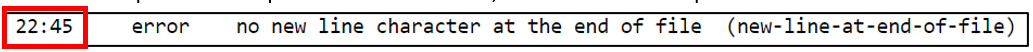
\includegraphics[width=16cm]{imagens/erro yaml.png}
	\caption{\label{fig:erroyaml} Exemplo de erro no yaml}
	\fonte{Os autores}
\end{figure}
\FloatBarrier

Elas representam, respectivamente, a linha e o caractere que apresentou o erro (ex: linha 22, caractere 45).


Esses foram os erros que conseguimos identificar conforme íamos tentando validar o nosso arquivo, então pode ser que há outros erros que não foram mapeados nessa postagem. 

Estamos abertos para a troca de experiências e esperamos ter ajudado :)

\section{Resumo de Atividades - Semana 11}
Na décima-primeira semana, entregamos e mostramos o documento final para o professor, que apontou alguns pontos de melhoria. Ele também alegou que o nosso arquivo equipe.yaml estava errado, pois não estava aparecendo no site da disciplina. Então fomos buscar mais a fundo sobre isso e conseguimos identificar os principais erros que podem aparecer na hora de validar um arquivo yaml. Assim, elaboramos um documento com esses principais erros, até mesmo para ajudar as próximas turmas da disciplina. 

No nosso checkpoint semanal, foi feito uma lista do que faltava para a aplicação ficar pronta e decidimos os próximos passos para cada integrante, que seria voltada para os ajustes no documento ou finalização da aplicação.

Além disso, ficamos sabendo que seríamos a primeira equipe a se apresentar (dia 26/07), então nos reunimos duas vezes para validar se estava tudo certo e também treinar para a apresentação final. 

Segue abaixo as atividades de cada integrante:

\begin{itemize}
\item André: fez a listagem de atividades e envio de anexos, a criação das conquistas, a entrega de atividades e de conquistas, o encerramento de turmas, correção na criação de atividades e o ranking
\item Bianca: ajustou o equipe.yaml, criou o documento dos erros do yaml, fez a apresentação do projeto e ajustou o documento final (segurança, escopo, manutenibilidade, métricas e apêndices)
\item Gustavo: fez a validação dos formulários de atividades e correções dos erros para a apresentação
\item Luiz: fez a geração do Latexdiff e os ajustes na documentação final (links de acesso, modelagem de dados, manutenibilidade, tecnologias e escopo)
\item Natan: gerou o vídeo do Gource, auxiliou na geração do Latexdiff e criou buscas dinâmicas dos registros da visão do administrador e do professor na tela do gestor
\item Patricia: fez os teste de alunos, de turmas, de conquistas e de atividades, o isolamento do firebase, a reorganização e a elaboração do roteiro de testes e montagem do backlog de correções
\end{itemize}

% ----------------------------------------------------------
\chapter{Protótipos das Telas}
\label{prototipos}
% ----------------------------------------------------------

\begin{figure}[htb]
    \centering
	
\includegraphics[width=16cm]{imagens/Geral-Login.png}
	\caption{\label{fig:login} Protótipo da Tela: Tela de Login}
	\fonte{Os autores}
\end{figure}
\FloatBarrier


\section{Visão do Administrador}

\begin{figure}[htb]
    \centering
	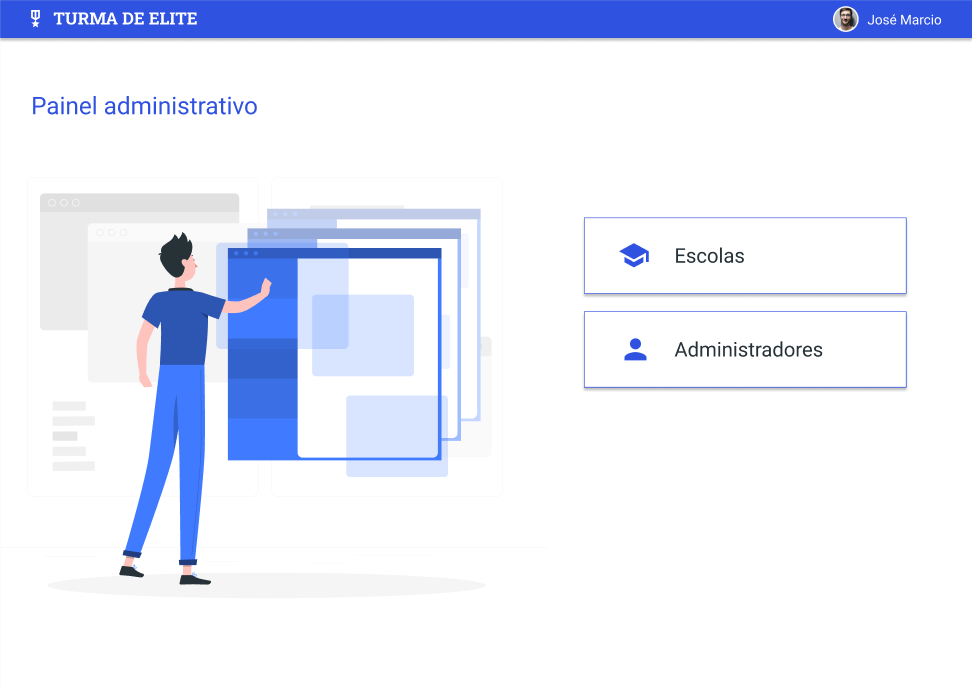
\includegraphics[width=16cm]{imagens/Administrador-PaginaInicial.png}
	\caption{\label{fig:administrador} Protótipo da Tela: Visão do Administrador - Página Inicial}
	\fonte{Os autores}
\end{figure}
\FloatBarrier

\begin{figure}[htb]
    \centering
	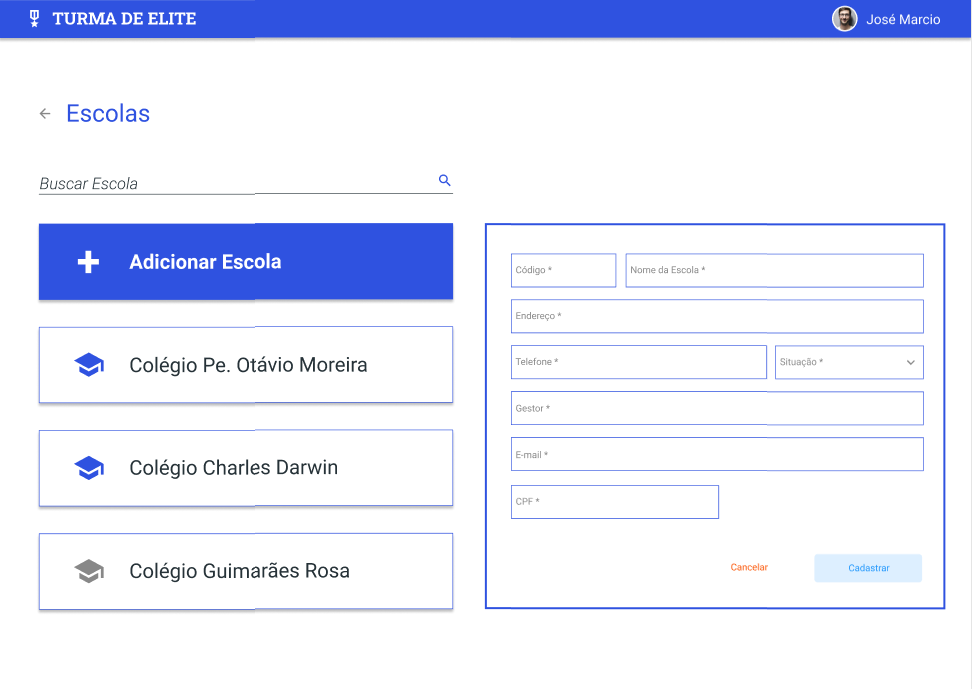
\includegraphics[width=16cm]{imagens/Administrador-CadastroEscola.png}
	\caption{\label{fig:cadastro-escola} Protótipo da Tela: Visão do Administrador - Cadastro de Escolas}
	\fonte{Os autores}
\end{figure}
\FloatBarrier

\begin{figure}[htb]
    \centering
	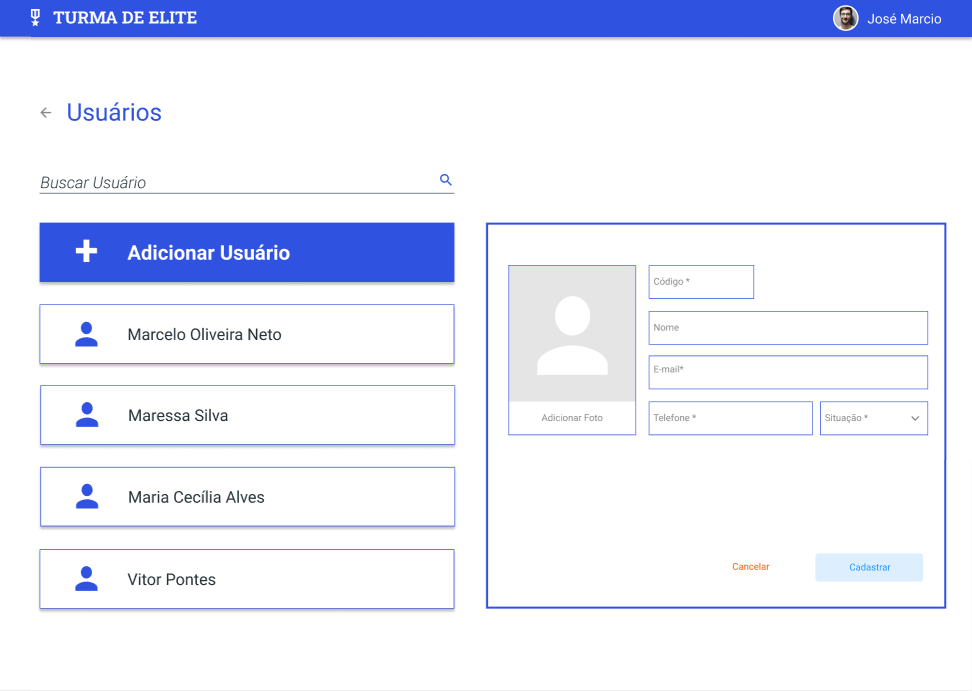
\includegraphics[width=16cm]{imagens/Administrador-CadastroUsuario.png}
	\caption{\label{fig:cadastro-usuário} Protótipo da Tela: Visão do Administrador - Cadastro de Usuários}
	\fonte{Os autores}
\end{figure}
\FloatBarrier


\section{Visão do Professor}

\begin{figure}[htb]
    \centering
	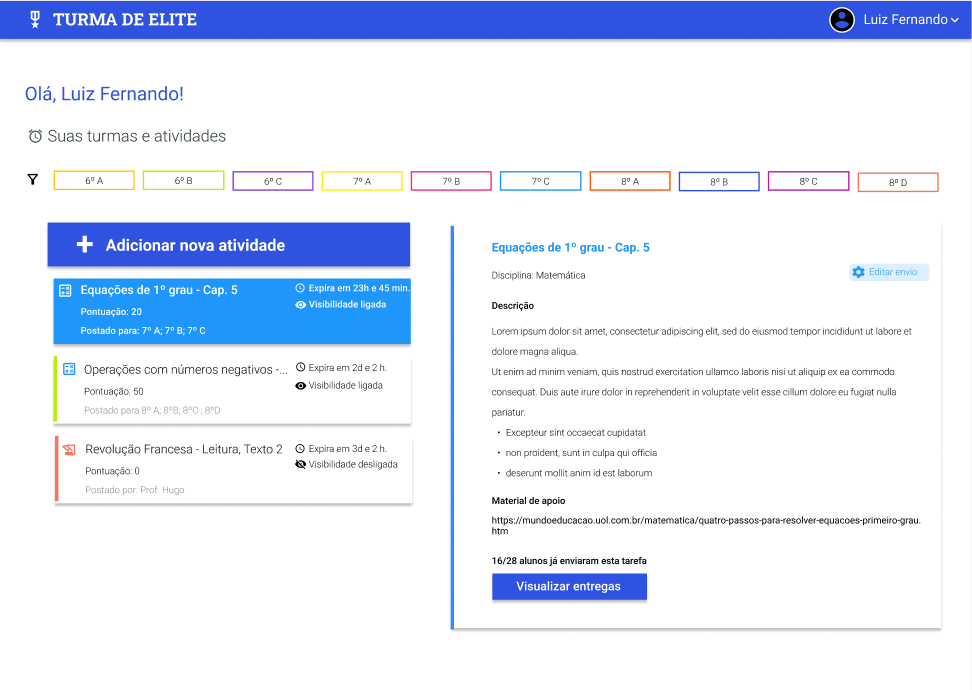
\includegraphics[width=16cm]{imagens/Professor-Atividades.png}
	\caption{\label{fig:atividades} Protótipo da Tela: Visão do Professor - Atividades}
	\fonte{Os autores}
\end{figure}
\FloatBarrier

\begin{figure}[htb]
    \centering
	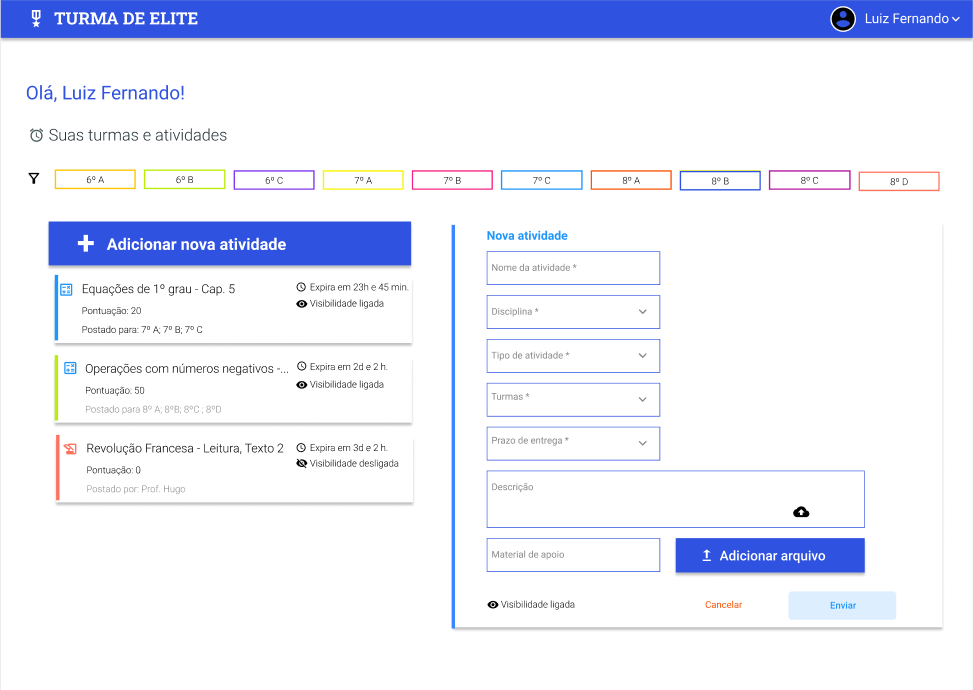
\includegraphics[width=16cm]{imagens/Professor-CadastroAtividades.png}
	\caption{\label{fig:professor} Protótipo da Tela: Visão do Professor - Cadastro de Atividades}
	\fonte{Os autores}
\end{figure}
\FloatBarrier


\section{Visão do Aluno}

\begin{figure}[htb]
    \centering
	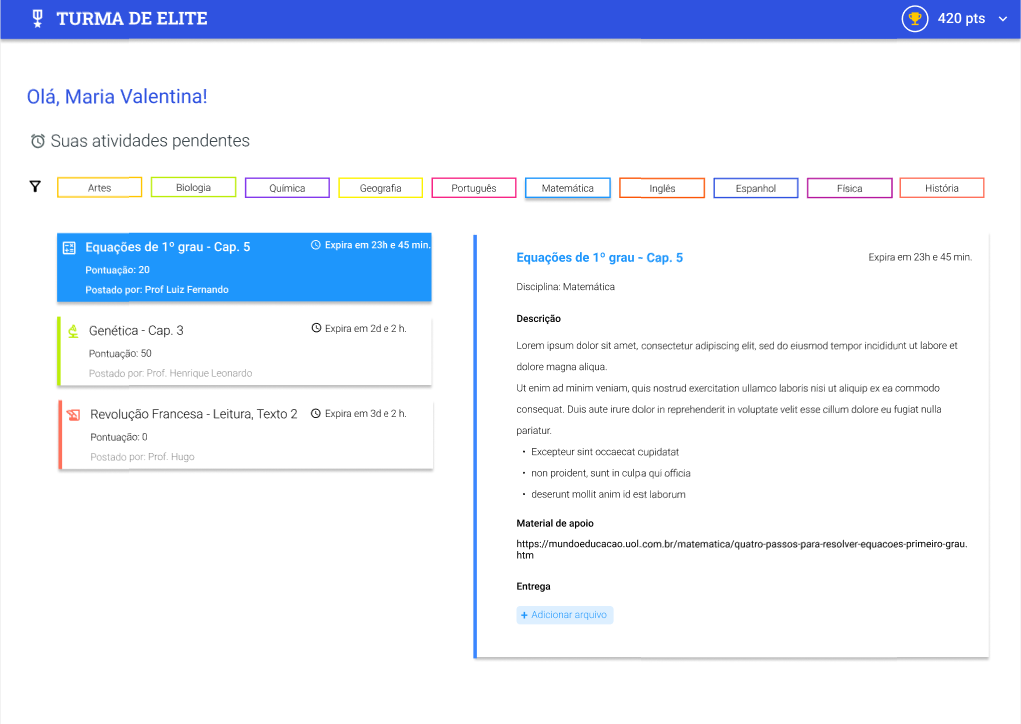
\includegraphics[width=16cm]{imagens/Aluno-Atividades.png}
	\caption{\label{fig:aluno} Protótipo da Tela: Visão do Aluno - Atividades}
	\fonte{Os autores}
\end{figure}
\FloatBarrier

\begin{figure}[htb]
    \centering
	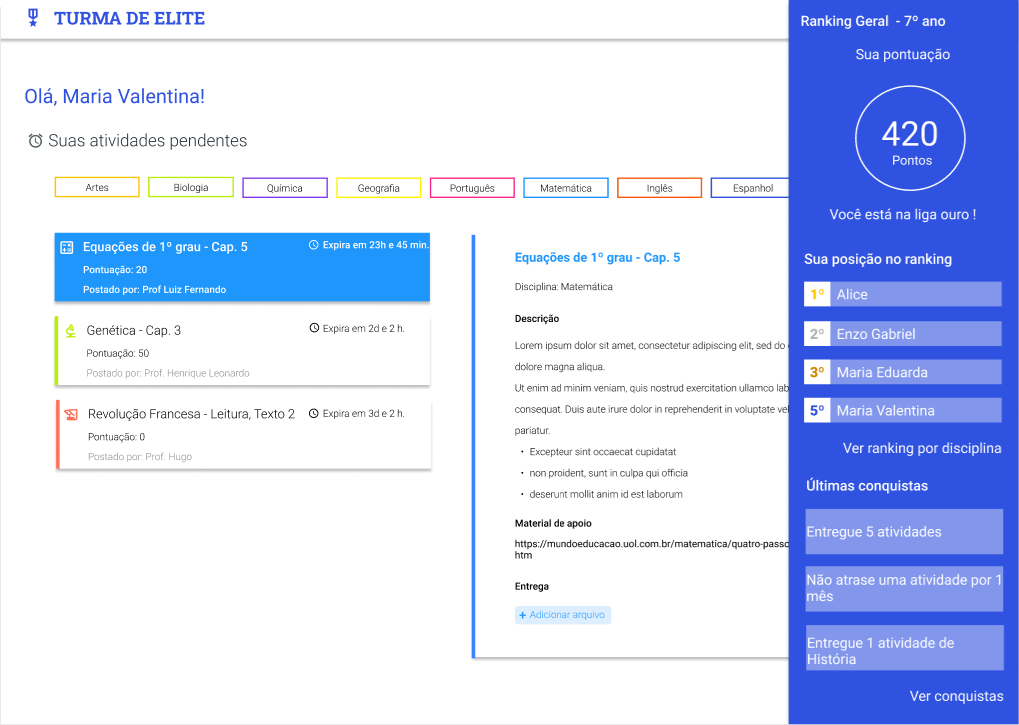
\includegraphics[width=16cm]{imagens/Aluno-MenuLateral.png}
	\caption{\label{fig:menu-lateral} Protótipo da Tela: Visão do Aluno - Menu Lateral}
	\fonte{Os autores}
\end{figure}
\FloatBarrier

\begin{figure}[htb]
    \centering
	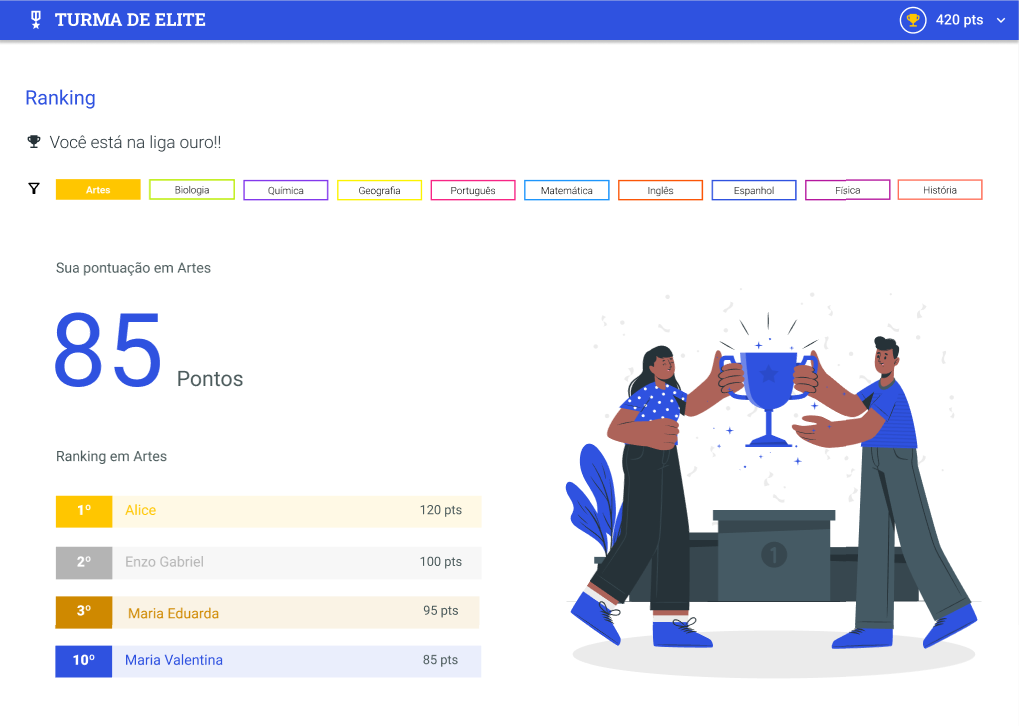
\includegraphics[width=16cm]{imagens/Aluno-Ranking.png}
	\caption{\label{fig:ranking} Protótipo da Tela: Visão do Aluno - Ranking}
	\fonte{Os autores}
\end{figure}
\FloatBarrier

\begin{figure}[htb]
    \centering
	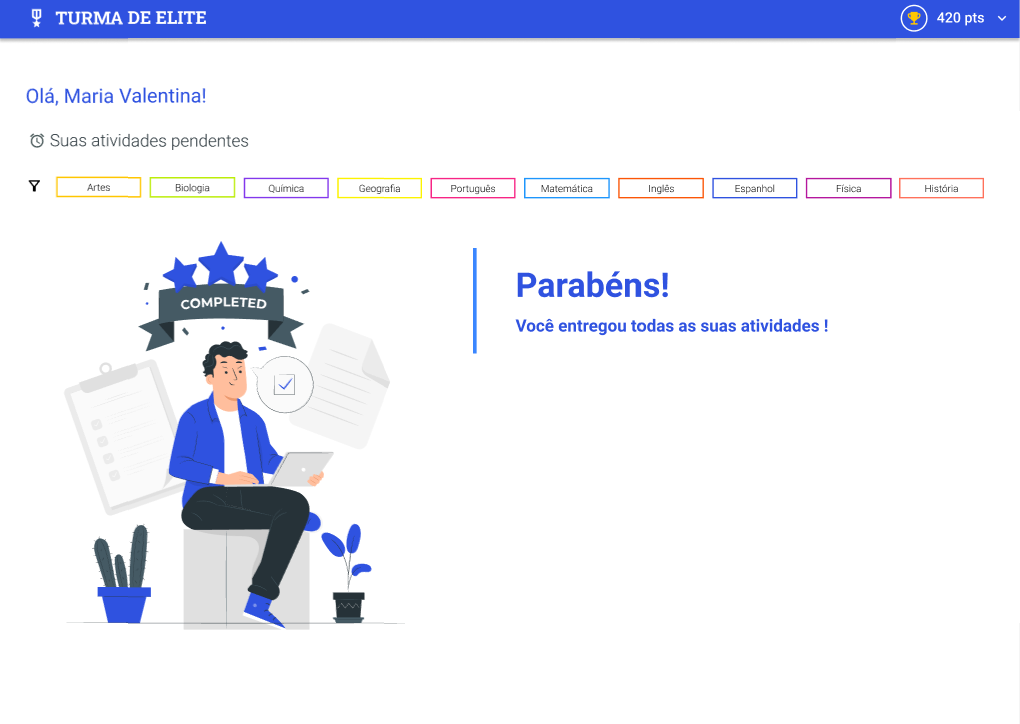
\includegraphics[width=16cm]{imagens/Aluno-Conquista.png}
	\caption{\label{fig:conquista} Protótipo da Tela: Visão do Aluno - Conquistas}
	\fonte{Os autores}
\end{figure}
\FloatBarrier

% ----------------------------------------------------------
\chapter{Entregáveis de modelagem}
% ----------------------------------------------------------
\section{\textit{Product Backlog}}
 {\pdfpagewidth=2\pdfpagewidth
%\thispagestyle{empty}
    \vspace*{-2cm}
    \noindent\parbox{\textwidth}{%
    \noindent\rlap{\includegraphics[width=388mm,height=216mm,page=2]{imagens/User Story Mapping FrameworkHD.jpg}}\endgraf
    \vspace{2ex}%
    \captionof{figure}{\label{product-backlog-apendice}Product Backlog}}
    \fonte{Os autores}
     \par
     \vspace*{-5cm}
     
\clearpage
}
\FloatBarrier

\section{Modelo Entidade Relacionamento}
 {\pdfpagewidth=2\pdfpagewidth
%\thispagestyle{empty}
    \vspace*{-2cm}
    \noindent\parbox{\textwidth}{%
    \noindent\rlap{\includegraphics[width=338mm,height=229mm,page=2]{imagens/ModeloConceitual.png}}\endgraf
    \vspace{2ex}%
    \captionof{figure}{\label{mer-apendice}Modelo Entidade Relacionamento}}
    \fonte{Os autores}
     \par
     \vspace*{-5cm}
     
\clearpage
}
\FloatBarrier

\section{Diagrama Entidade Relacionamento}

 {\pdfpagewidth=2\pdfpagewidth
%\thispagestyle{empty}
    \vspace*{-2cm}
    \noindent\parbox{\textwidth}{%
    \noindent\rlap{\includegraphics[width=308mm,height=229mm,page=2]{imagens/dernovo.png}}\endgraf
    \vspace{2ex}%
    \captionof{figure}{\label{der-apendice}Diagrama Entidade Relacionamento}}
    \fonte{Os autores}
     \par
     \vspace*{-5cm}
\clearpage
}
\FloatBarrier

% ----------------------------------------------------------
\chapter{SSL Test - Back-end}
\label{ssltest-backend}
% ----------------------------------------------------------
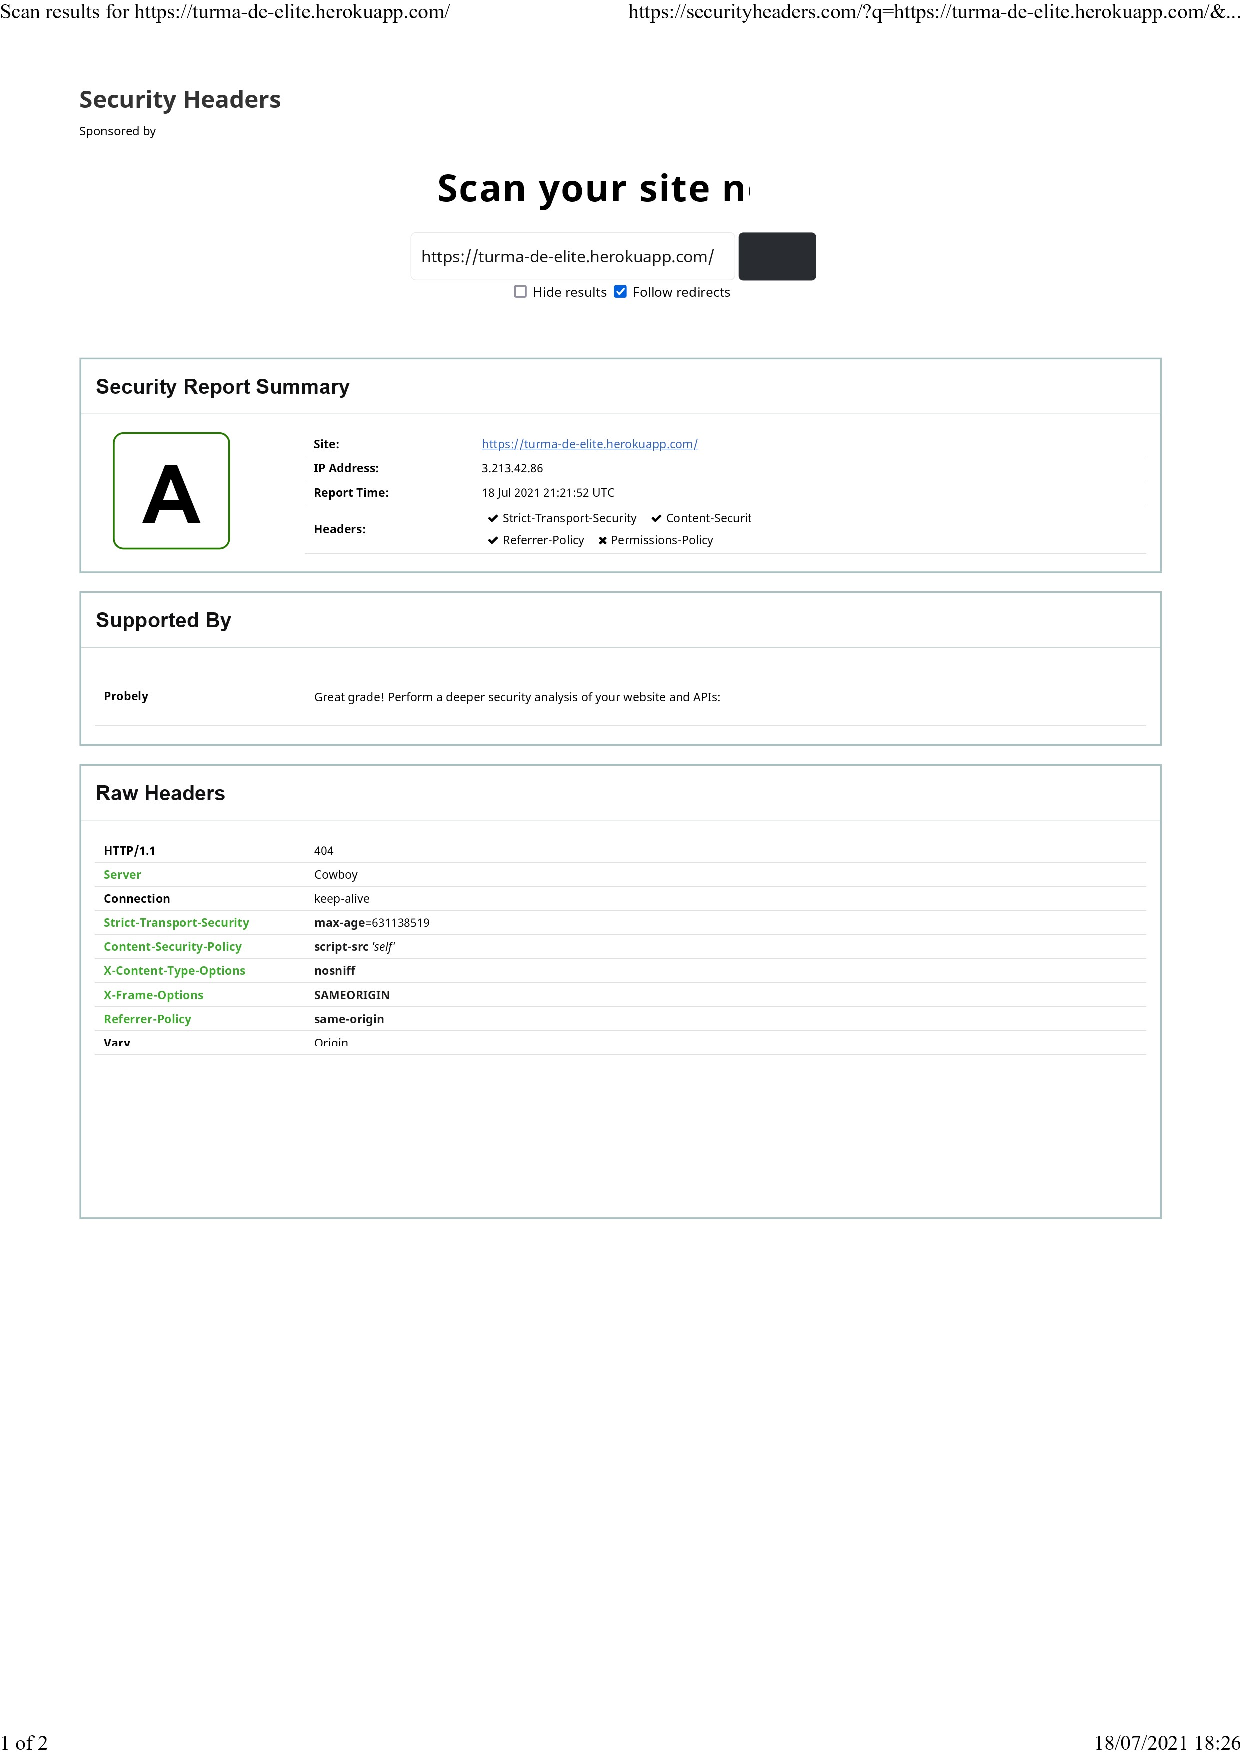
\includepdf[pages=-]{EntregaFinal/SECURITY_DOC.pdf}

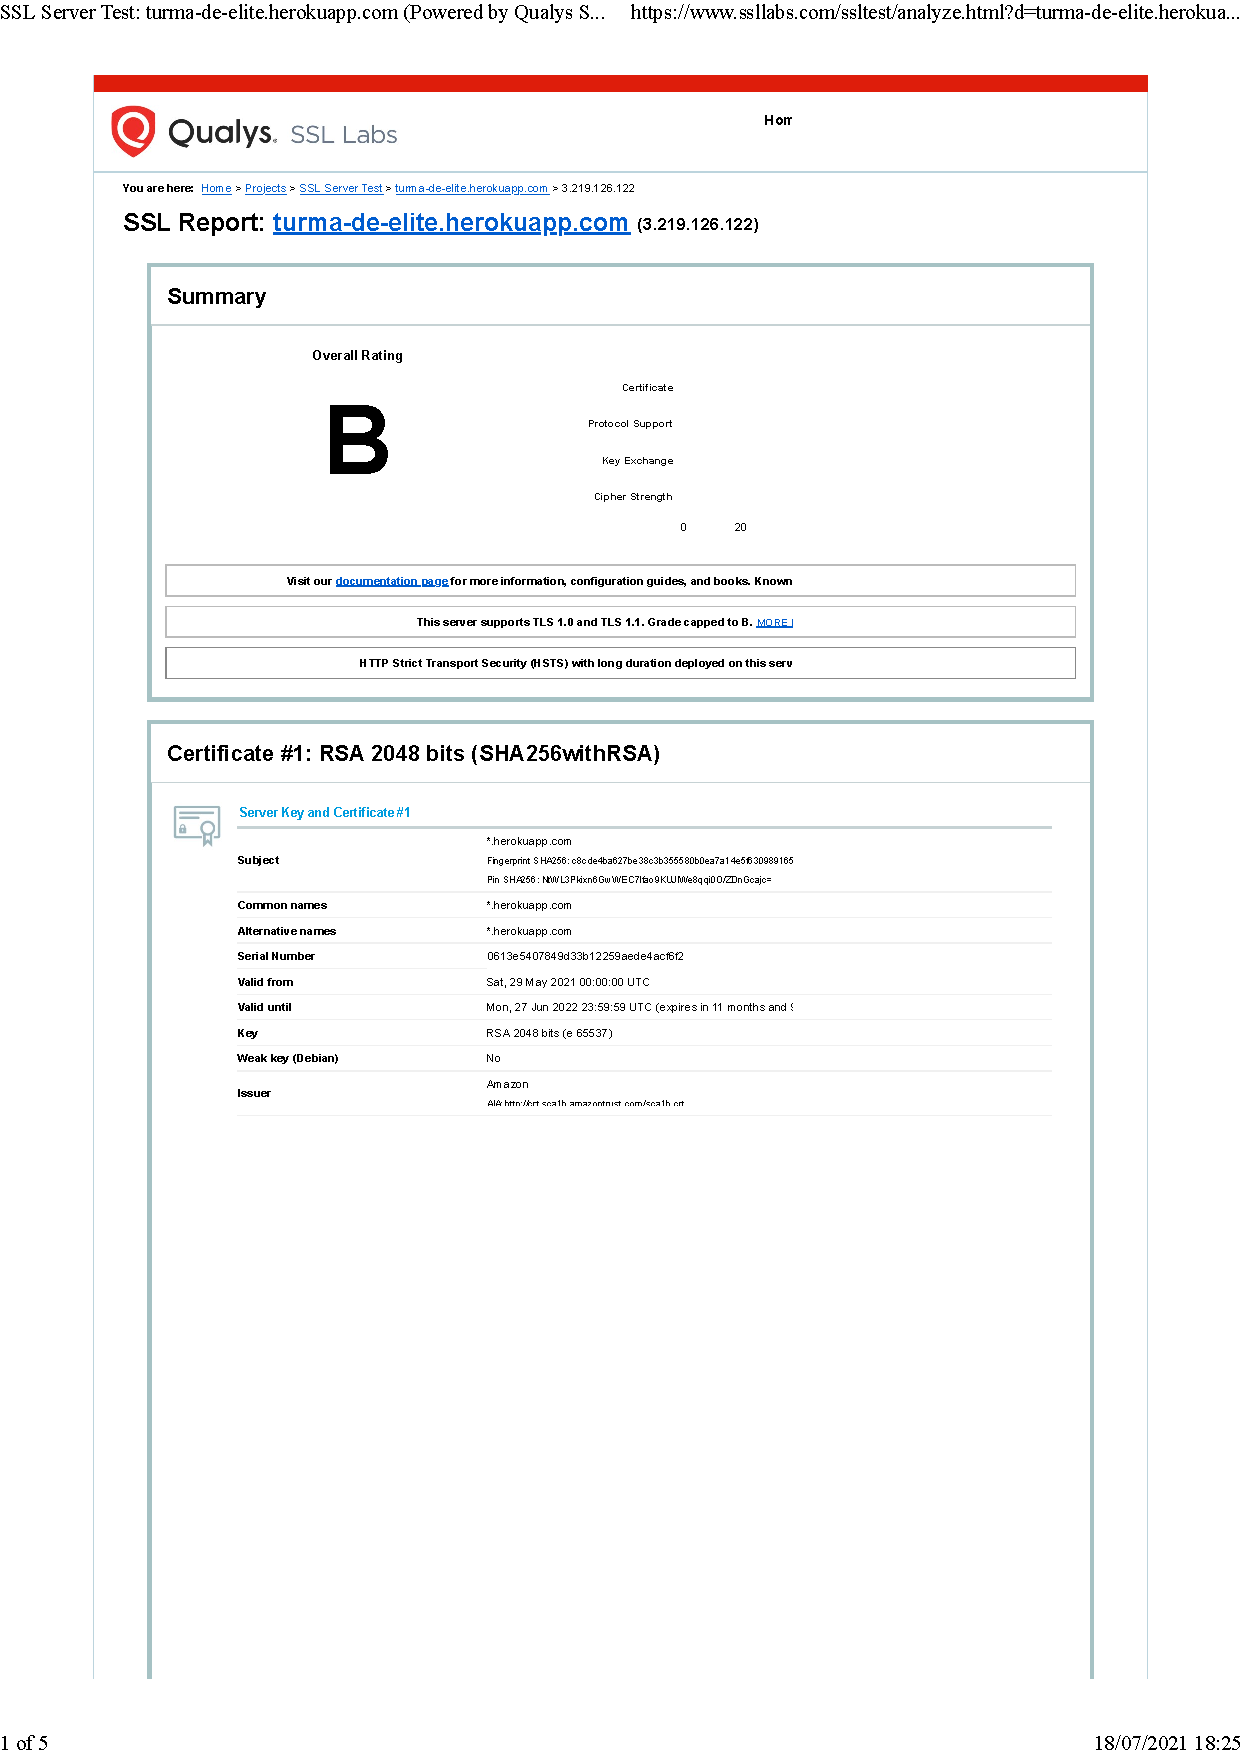
\includepdf[pages=-]{EntregaFinal/SSL_DOC.pdf}

% ----------------------------------------------------------
\chapter{SSL Test - Front-end}
\label{ssltest-frontend}
% ----------------------------------------------------------
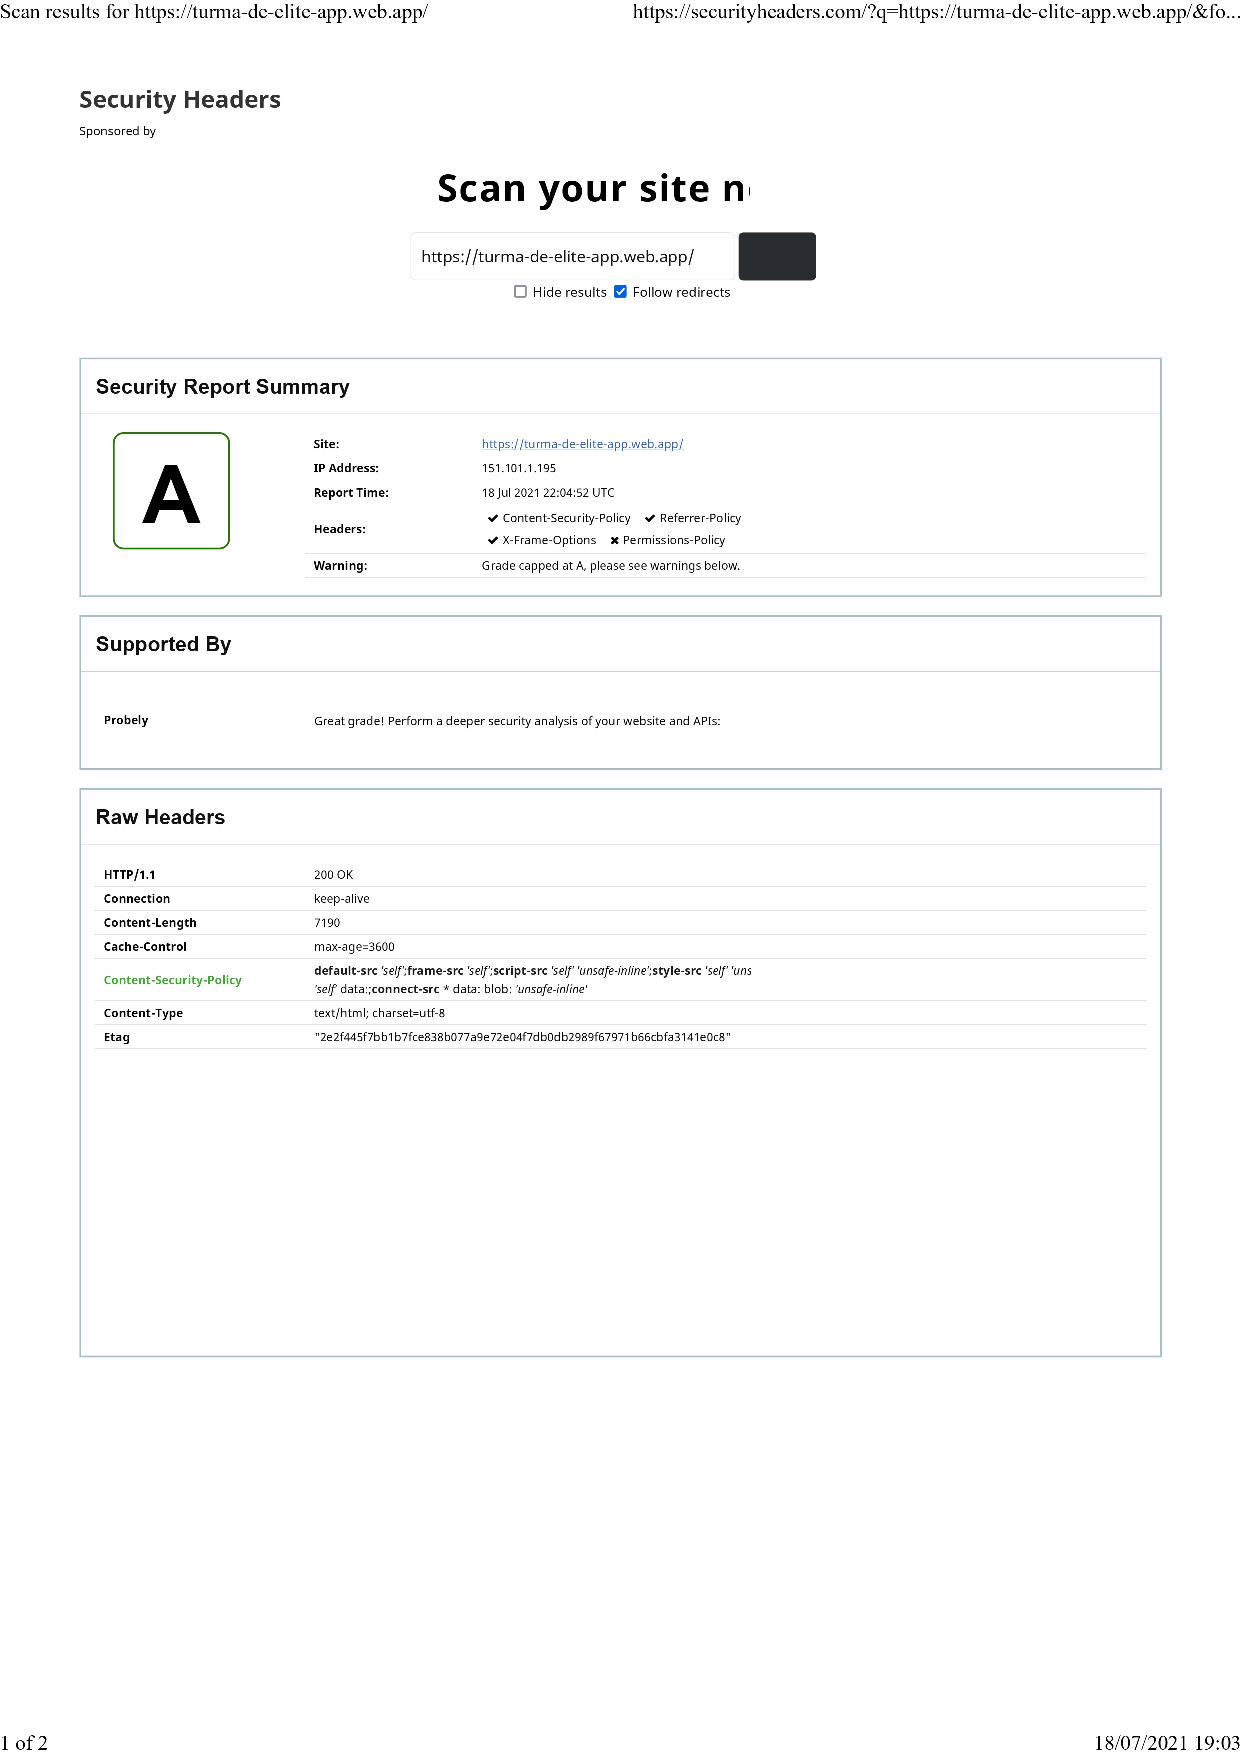
\includepdf[pages=-]{EntregaFinal/FRONT_END_SECURITY.pdf}

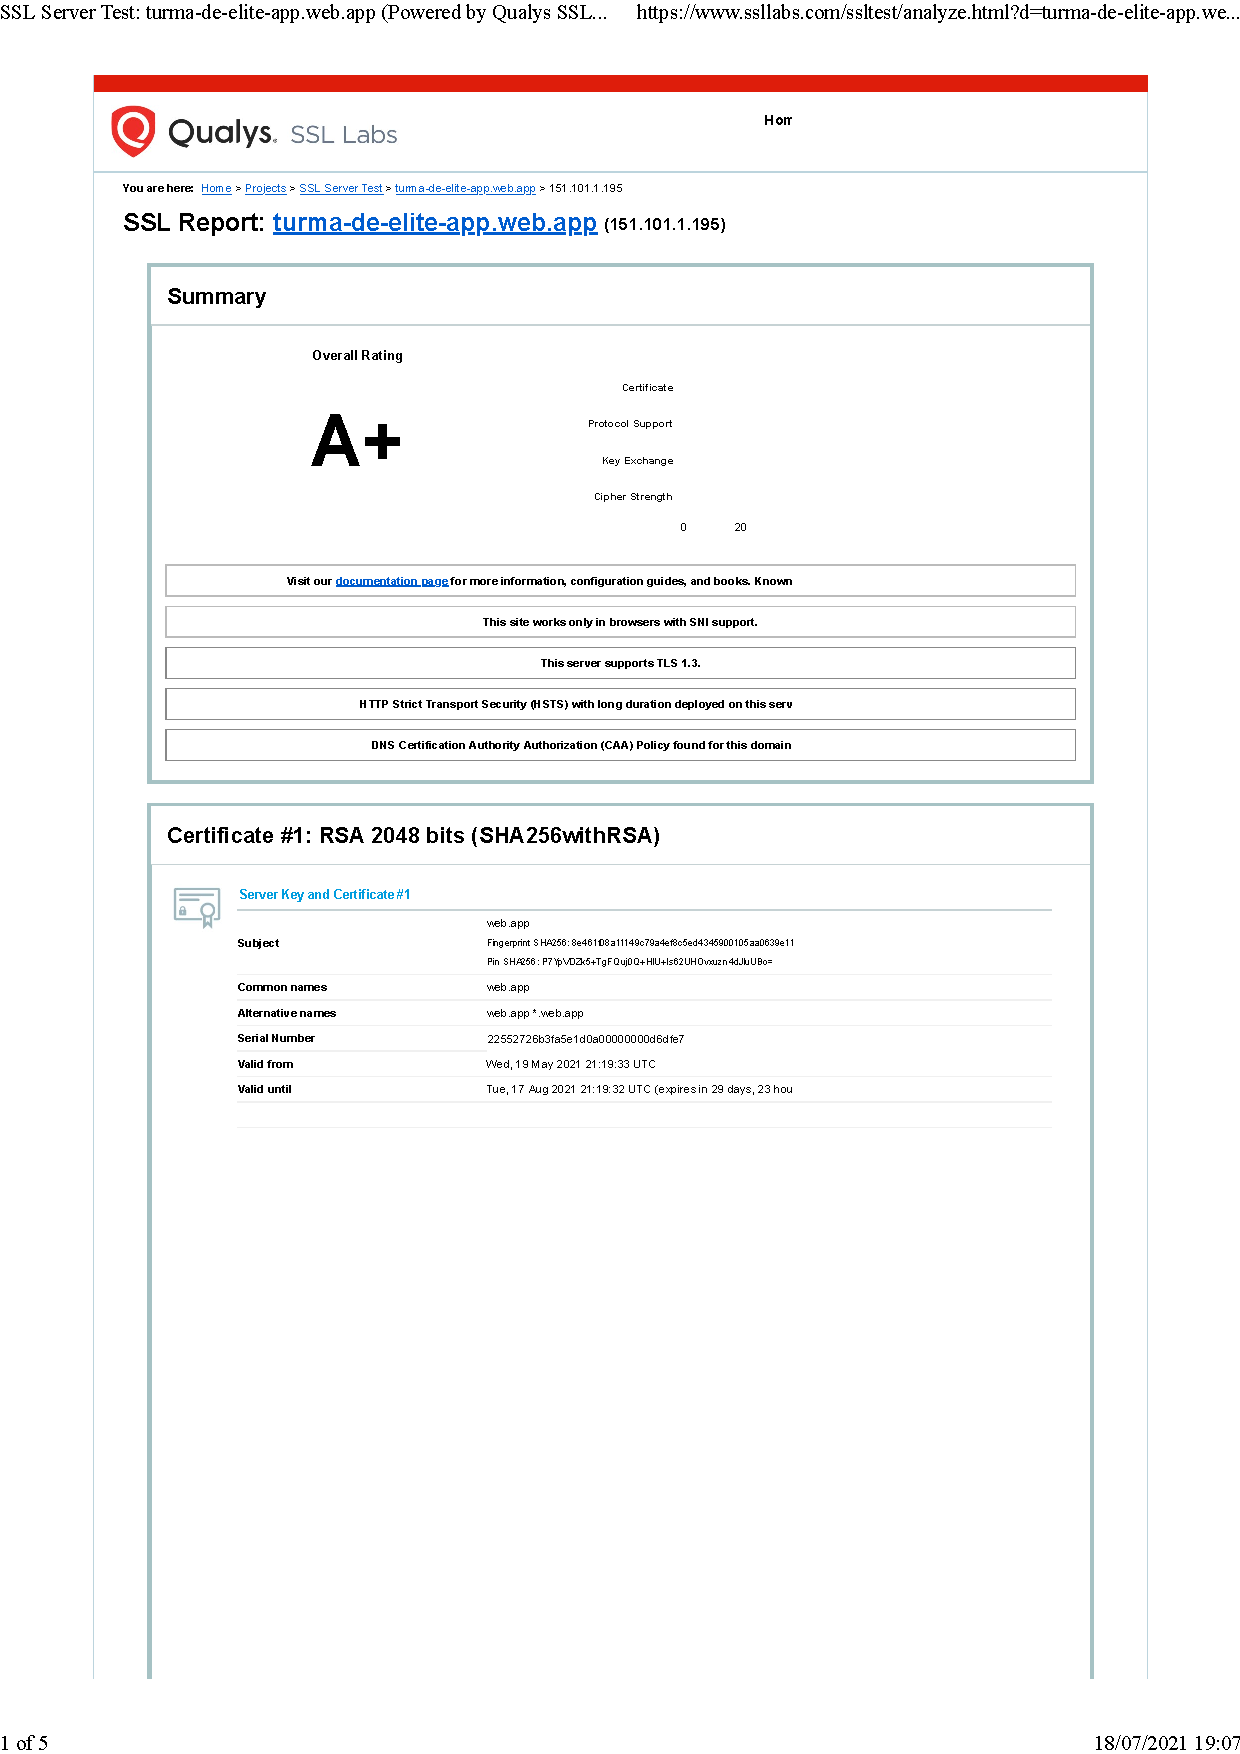
\includepdf[pages=-]{EntregaFinal/SSL_FRONT_DOC.pdf}
\end{apendicesenv}
% ---
